\chapter{Baadal Sandbox Setup Usage}

This chapter will provide the necessary commmands, interfaces and methodology to use baadal sandbox. We thought of including this as we spent much of the effort in understanding baadal system. There is no proper documentation on usage of baadal sandbox. Hence we put necessary screenshots in this chapter to enable others use baadal sandbox in convenient manner.

Following are the steps to start with sandbox server we established:-

\begin{enumerate}
    \item Login to server used for baadal sandbox setup
    
\begin{figure}[h]
\centering
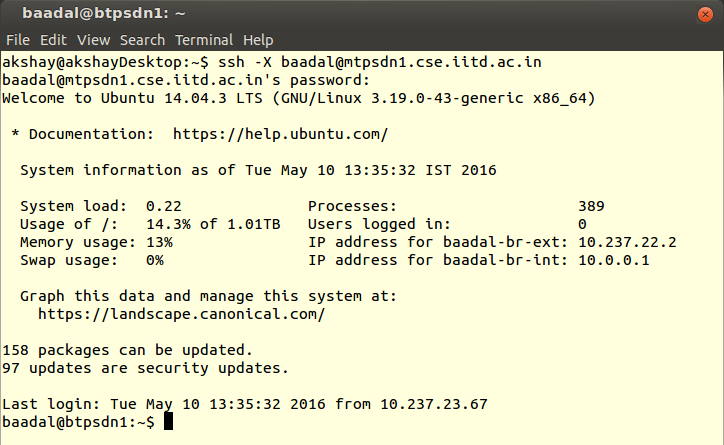
\includegraphics[width=0.9\textwidth]{first_login}
\caption{Login to the baadal sandbox server}
\end{figure}

\newpage
\item For status of VMs running in sandbox we can use \textit{sudo virsh list --all}
\begin{figure}[h]
\caption{Different VMs running in the sandbox}
\centering
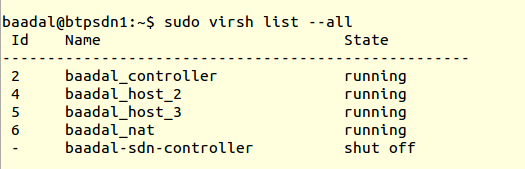
\includegraphics[width=0.9\textwidth]{Status_VMs}
\end{figure}


\item Using \textit{ifconfig} we can see the network configuration for the server.
\begin{figure}[h]
\caption{Output of ifconfig command on sandbox server}
\centering
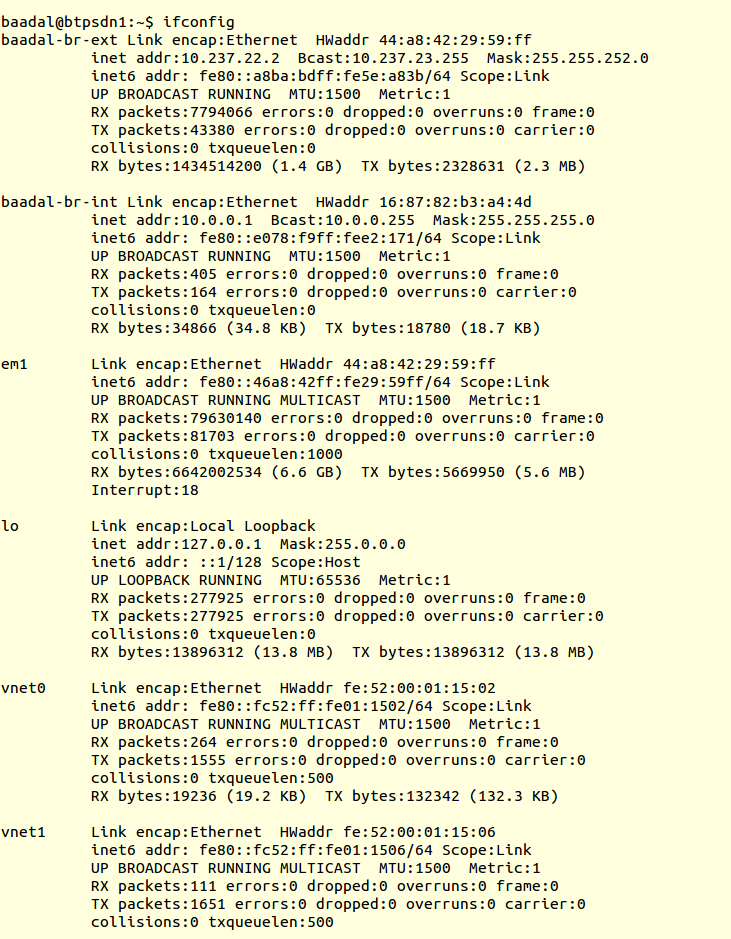
\includegraphics[height=10cm, width=0.9\textwidth]{ifconfig_server}
\end{figure}

\newpage
\item login inside the controller

\begin{figure}[h]
\caption{Login in the baadal controller}
\centering
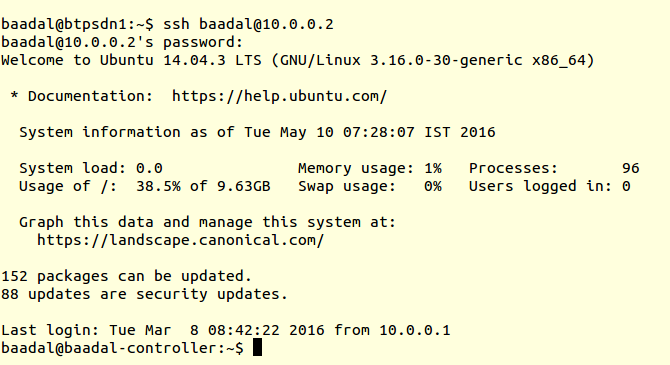
\includegraphics[height = 5cm, width=0.9\textwidth]{login_controller}
\end{figure}


\begin{figure}[h]
\caption{ifconfig showing 255 fake bridges inside the controller}
\centering
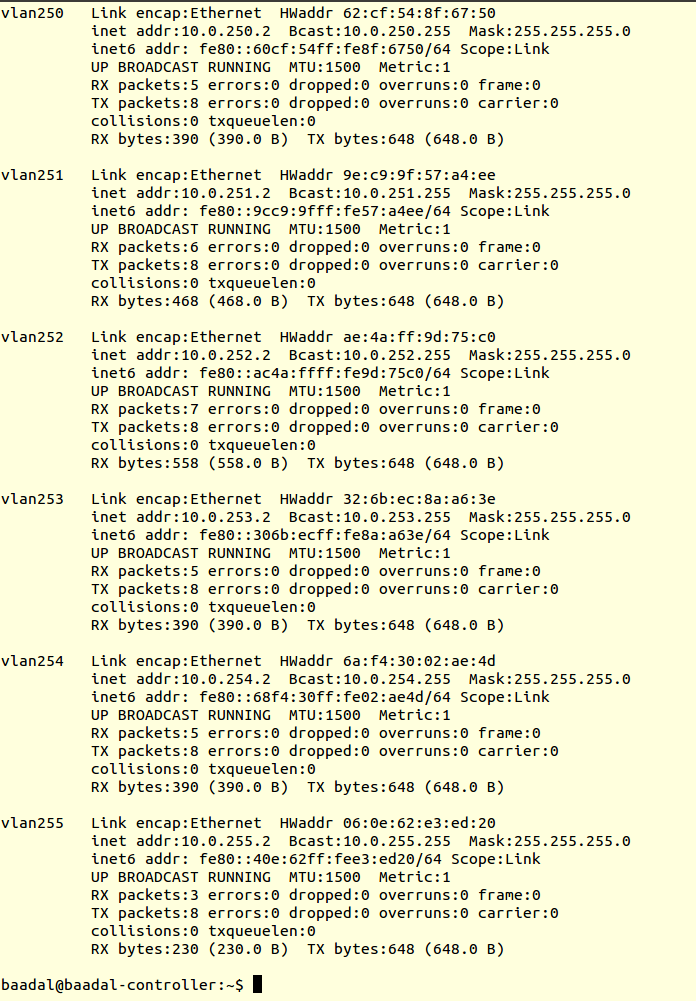
\includegraphics[height=9cm, width=0.9\textwidth]{ifconfig_controller}
\end{figure}

\begin{figure}
\caption{Web2py Processes Running inside controller}
\centering
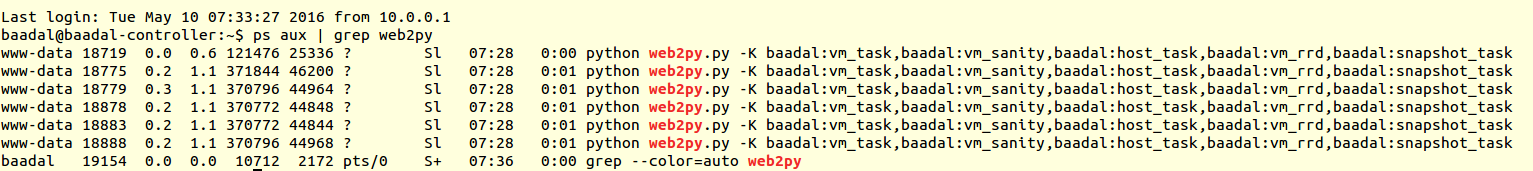
\includegraphics[height=2.5cm,width=0.9\textwidth]{web2py_processes_controller}
\end{figure}

\newpage
\item Login inside the nat is shown as

\begin{figure}[h]
\caption{Login inside the nat}
\centering
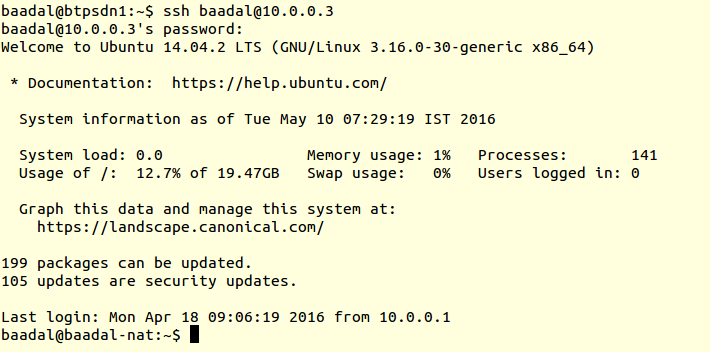
\includegraphics[width=0.9\textwidth]{login_nat}
\end{figure}


\begin{figure}[h]
\caption{ifconfig showing 255 fake bridges inside the NAT}
\centering
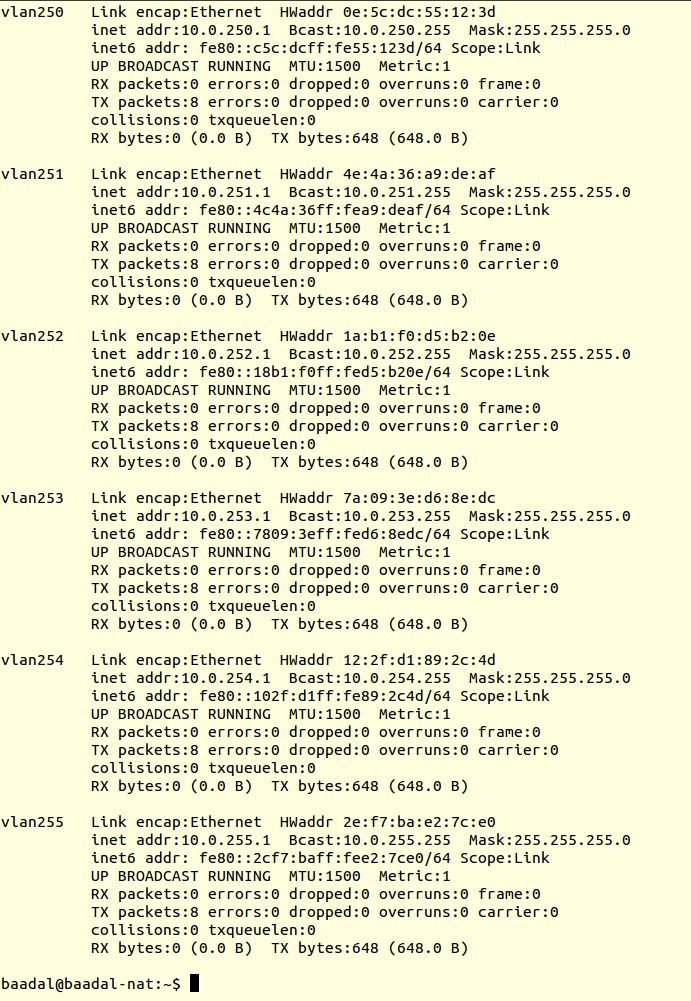
\includegraphics[width=0.9\textwidth]{ifconfig_nat}
\end{figure}

\item Login inside host

\begin{figure}[h]
\caption{Login inside host 10.0.0.6}
\centering
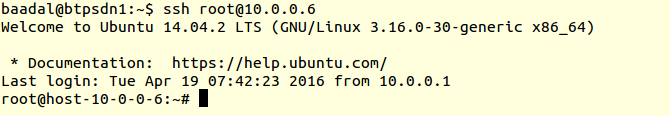
\includegraphics[width=0.9\textwidth]{login_host_6}
\end{figure}


\begin{figure}[h]
\caption{Network configuration of host 10.0.0.6}
\centering
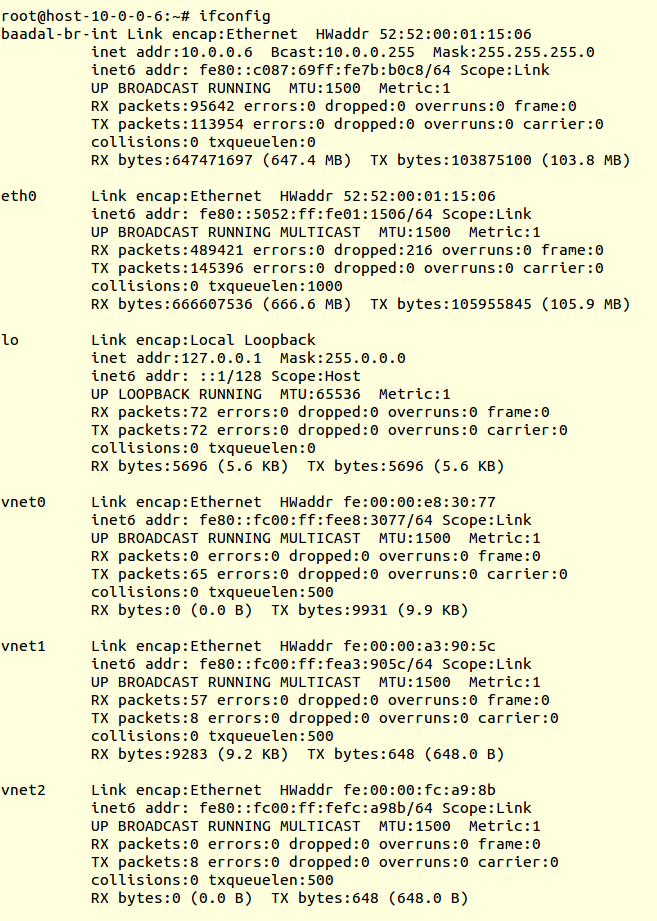
\includegraphics[width=0.9\textwidth]{ifconfig_host6}
\end{figure}

\begin{figure}[h]
\caption{Login inside host 10.0.0.7}
\centering
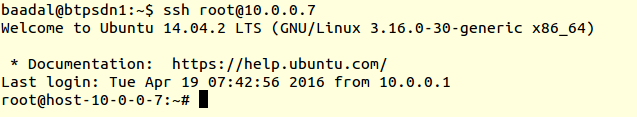
\includegraphics[width=0.9\textwidth]{login_host7}
\end{figure}


\begin{figure}[h]
\caption{Network configuration of host 10.0.0.6}
\centering
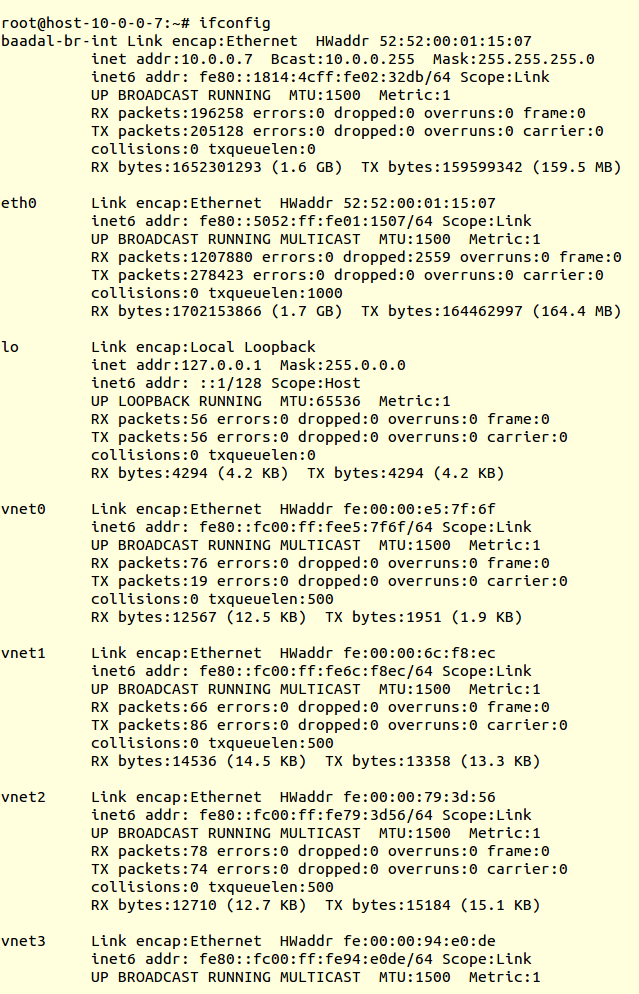
\includegraphics[width=0.9\textwidth]{ifconfig_host7}

\end{figure}

\item \textit{virsh list --all} shows the VMs running inside 10.0.0.6

\begin{figure}[h]
\caption{VMs shutdown status inside host 10.0.0.6}
\centering
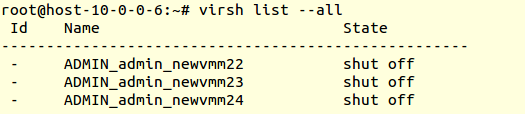
\includegraphics[width=0.9\textwidth]{host6_VMs_shutoff}

\end{figure}

\begin{figure}[h]
\caption{Starting VMs inside host 10.0.0.6}
\centering
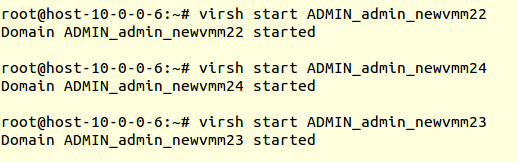
\includegraphics[width=0.9\textwidth]{host6_VMs_start}

\end{figure}

\begin{figure}[h]
\caption{Running VMs inside host 10.0.0.6}
\centering
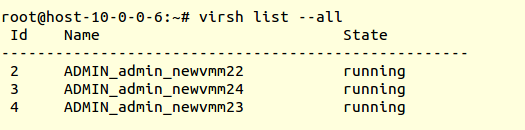
\includegraphics[width=0.9\textwidth]{host6_VMs_running}

\end{figure}

\item \textit{virsh list --all} shows the VMs running inside 10.0.0.7

\begin{figure}[h]
\caption{VMs shutdown status inside host 10.0.0.7}
\centering
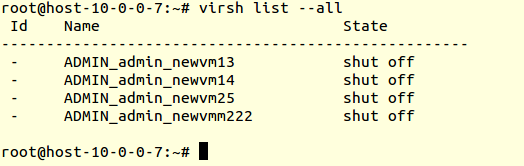
\includegraphics[width=0.9\textwidth]{host7_VMs_shutoff}

\end{figure}

\begin{figure}[h]
\caption{Starting VMs inside host 10.0.0.7}
\centering
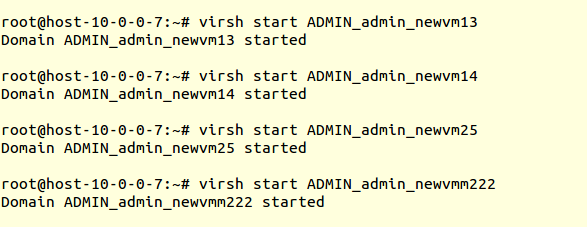
\includegraphics[width=0.9\textwidth]{host7_startinVMs}

\end{figure}

\begin{figure}[h]
\caption{Running VMs inside host 10.0.0.7}
\centering
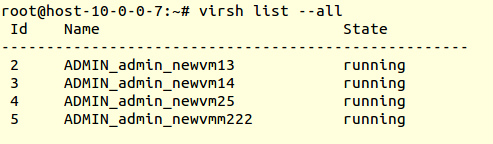
\includegraphics[width=0.9\textwidth]{host7_VMs_running}

\end{figure}

\item \textit{virt-viewer domain\_name} will open the GUI for the VM whose domain name is specified. Below figure shows for VM \textit{ADMIN\_admin\_newvm25}


\begin{figure}[h]
\caption{Console output for VM 10.0.4.25 after running virt-viewer}
\centering
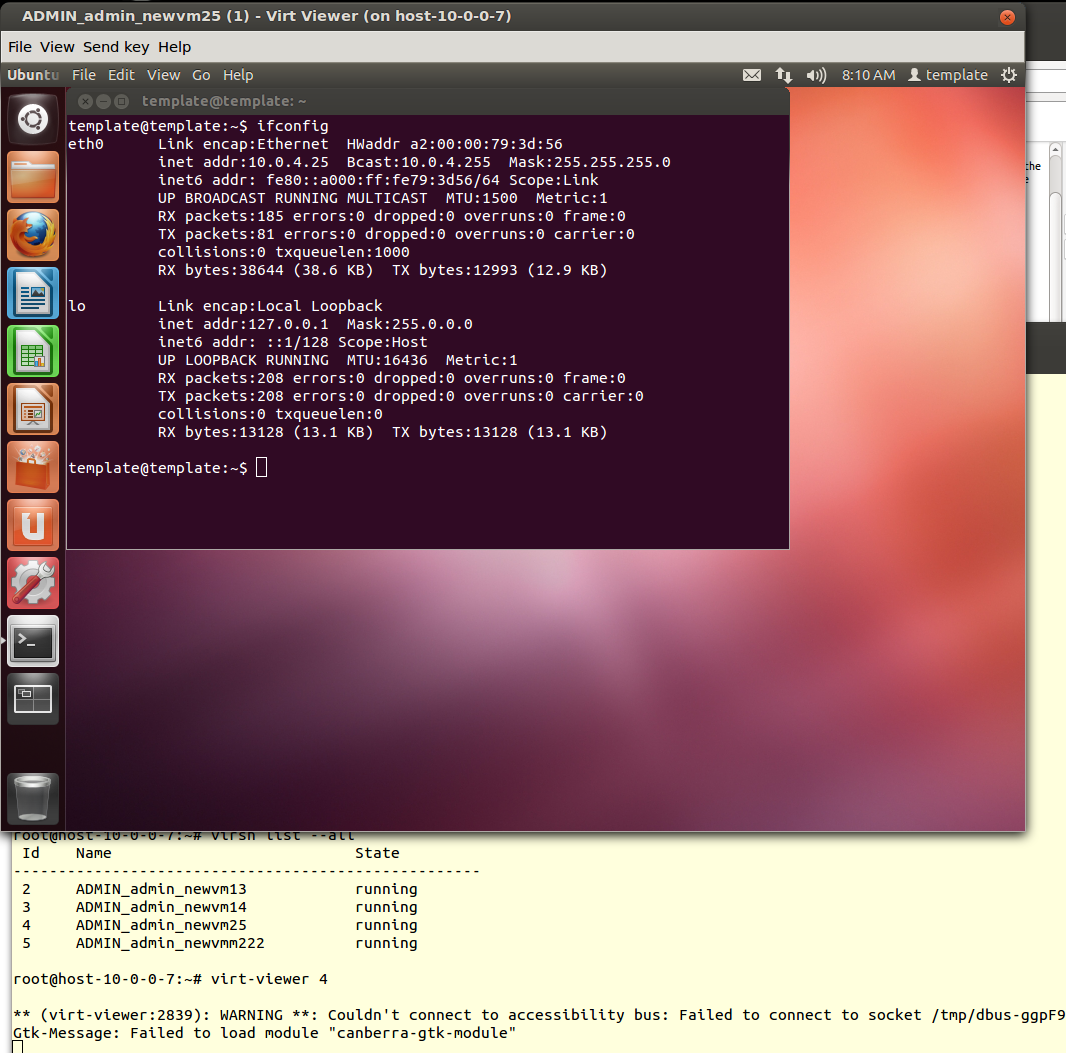
\includegraphics[width=0.9\textwidth]{virt_viewer_host7_ifconfig_425}
\end{figure}
\end{enumerate}